\documentclass[aspectratio=169,10pt,t,german,xcolor=table]{beamer}
\usepackage{../../common/beamer-cgs-lecture}

\title{Gem Illuminator}
\author{Pascal Lange, Sebastian Koall, Jennifer Stamm}
\institute{\translate{Hasso Plattner Institute}}
\date{WiSe~2014/2015}

\subtitle{Game Programming}
\titlegraphic{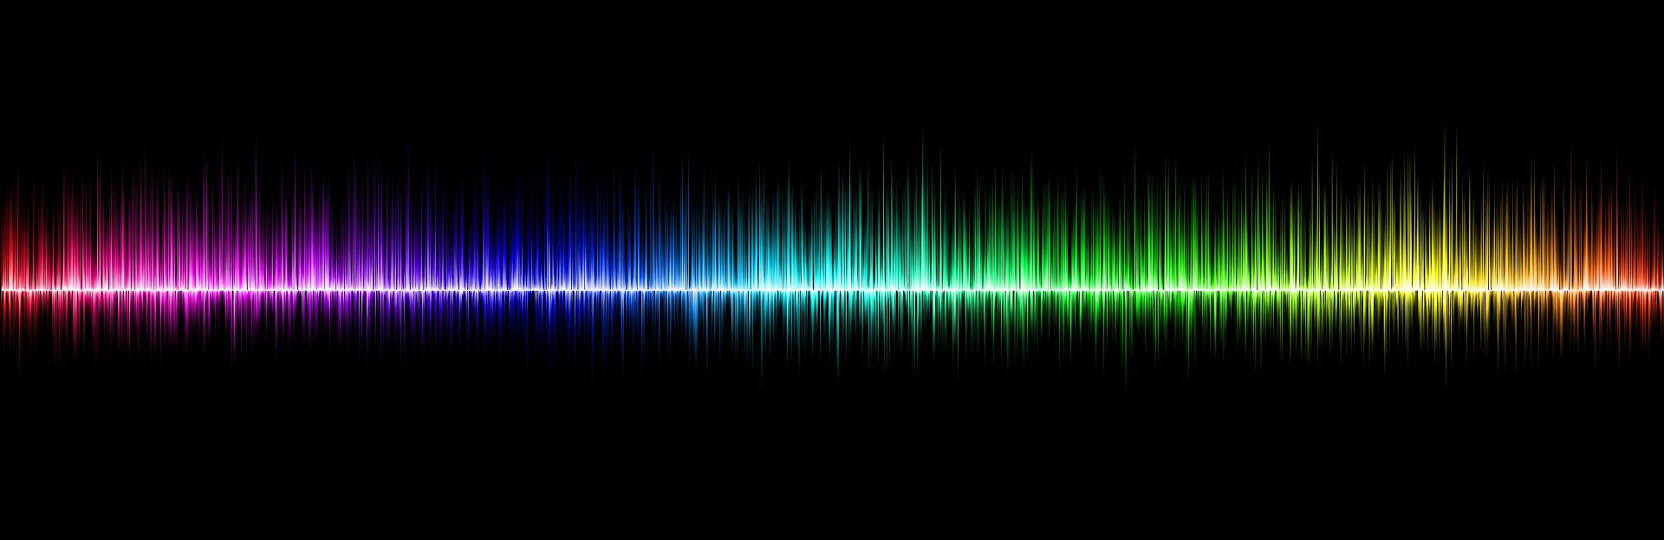
\includegraphics[width=\linewidth]{images/teaser}}

\begin{document}

\slidetitle
\section*{Zwischenstandspräsentation}

\begin{frame}{Demo}
	%TODO Aktueller Screenshot/Video
	\begin{figure}
		\centering
		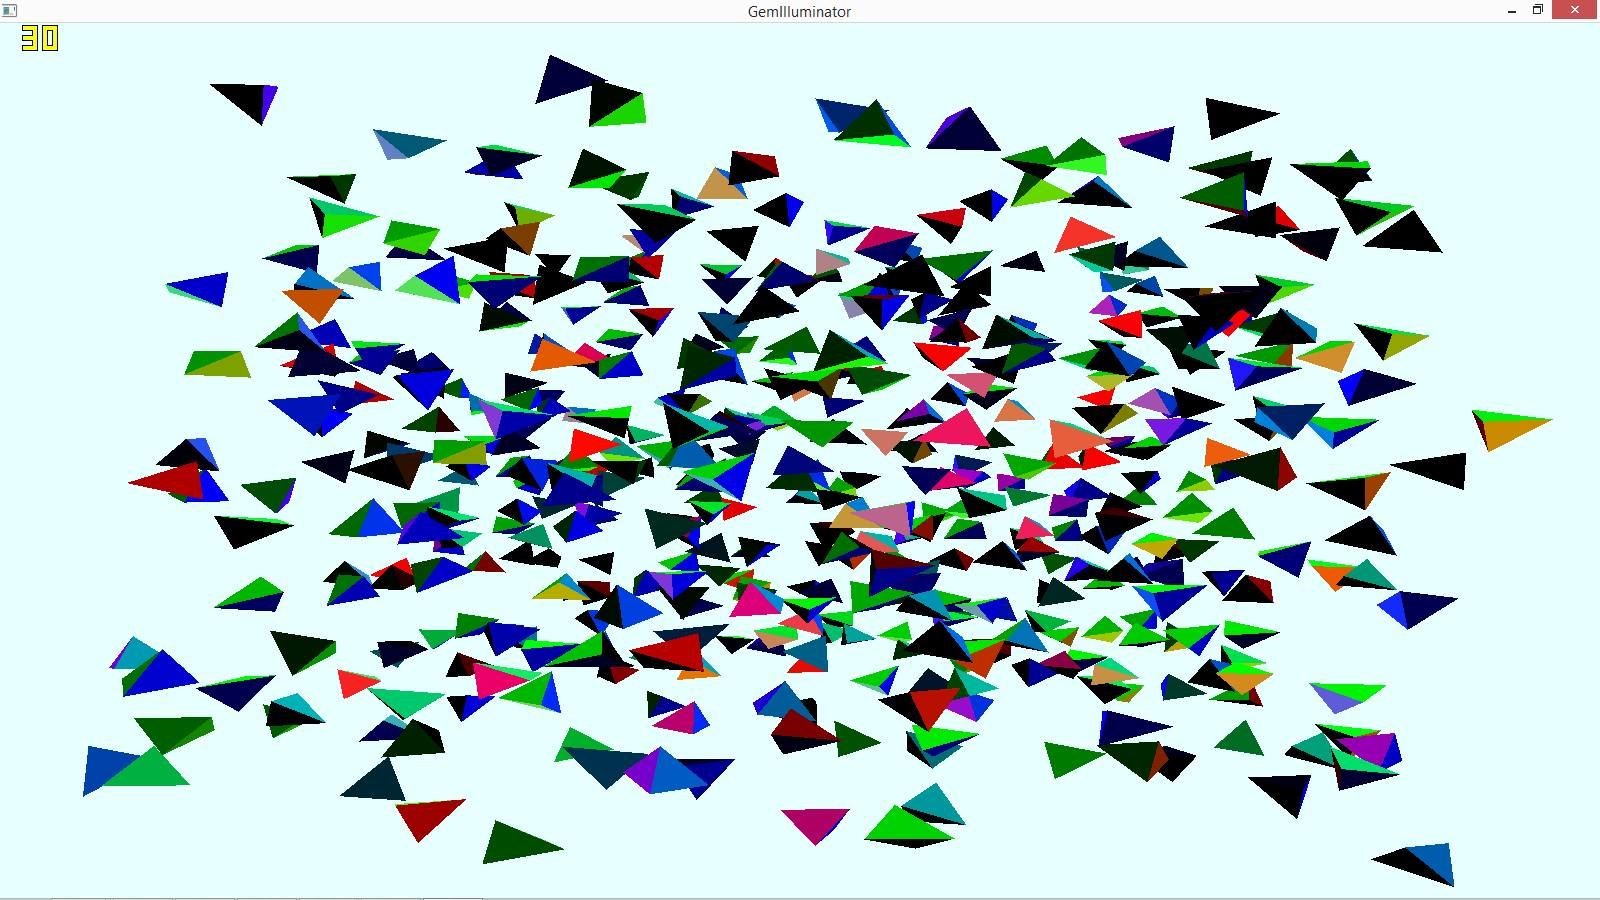
\includegraphics[width=\textwidth, height=0.7\textheight, keepaspectratio]{images/500_gems_intel}
	\end{figure}
\end{frame}


\begin{frame}{Architektur - C++}
	\begin{figure}
		\centering
		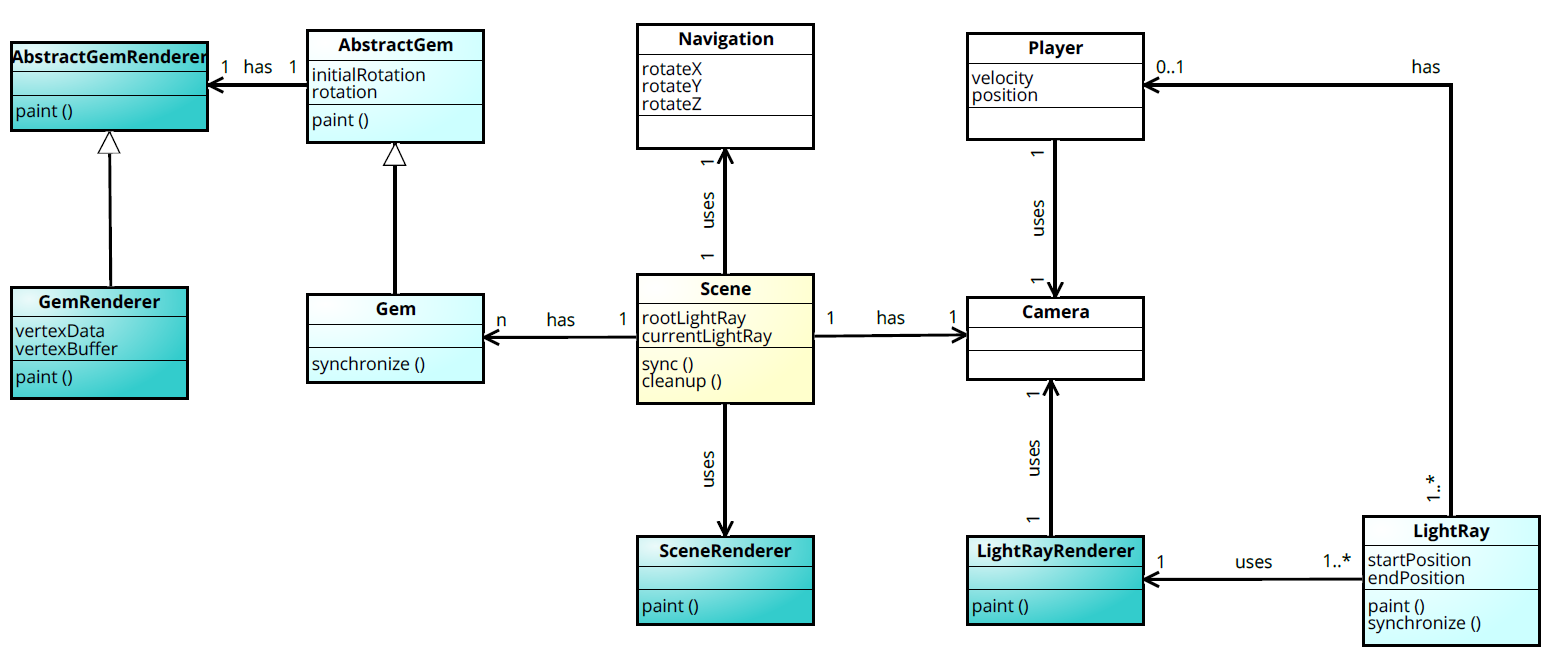
\includegraphics[width=\textwidth, height=\textheight, keepaspectratio]{images/klassendiagramm}
	\end{figure}
\end{frame}


\slideonetoone
{Herausforderungen}
{	
	\begin{figure}
		\centering
		\begin{subfigure}{\textwidth}
			\centering
			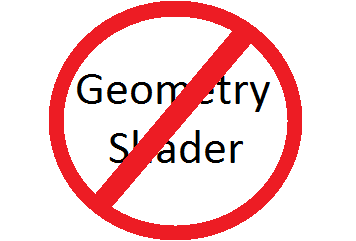
\includegraphics[width=\textwidth, height=0.35\textheight, keepaspectratio]{images/nogeometry}
			\caption{Normalenberechnung}
		\end{subfigure}
		\begin{subfigure}{\textwidth}
			\centering
			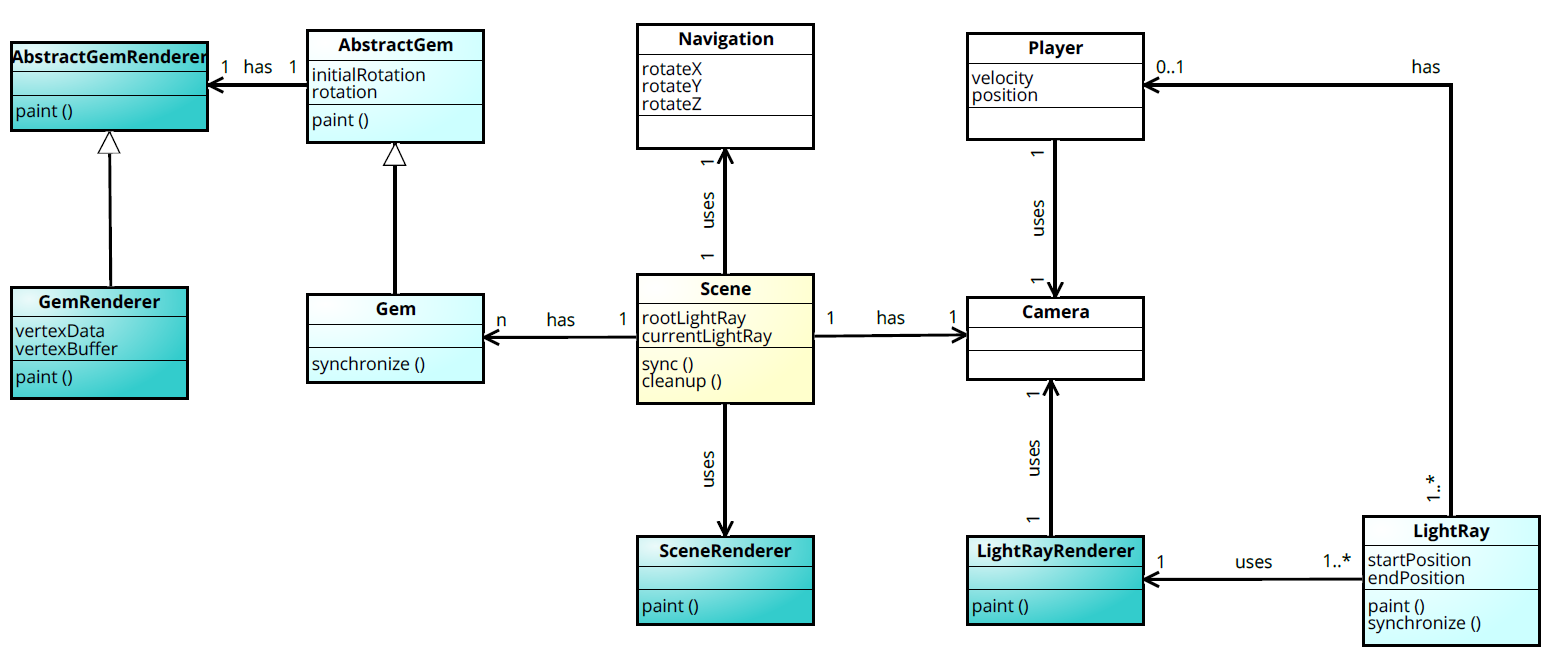
\includegraphics[width=\textwidth, height=0.35\textheight, keepaspectratio]{images/klassendiagramm}
			\caption{QML-Listenlimit}
		\end{subfigure}
	\end{figure}
}
{
	\begin{figure}
		\centering
		\begin{subfigure}{\textwidth}
			\centering
			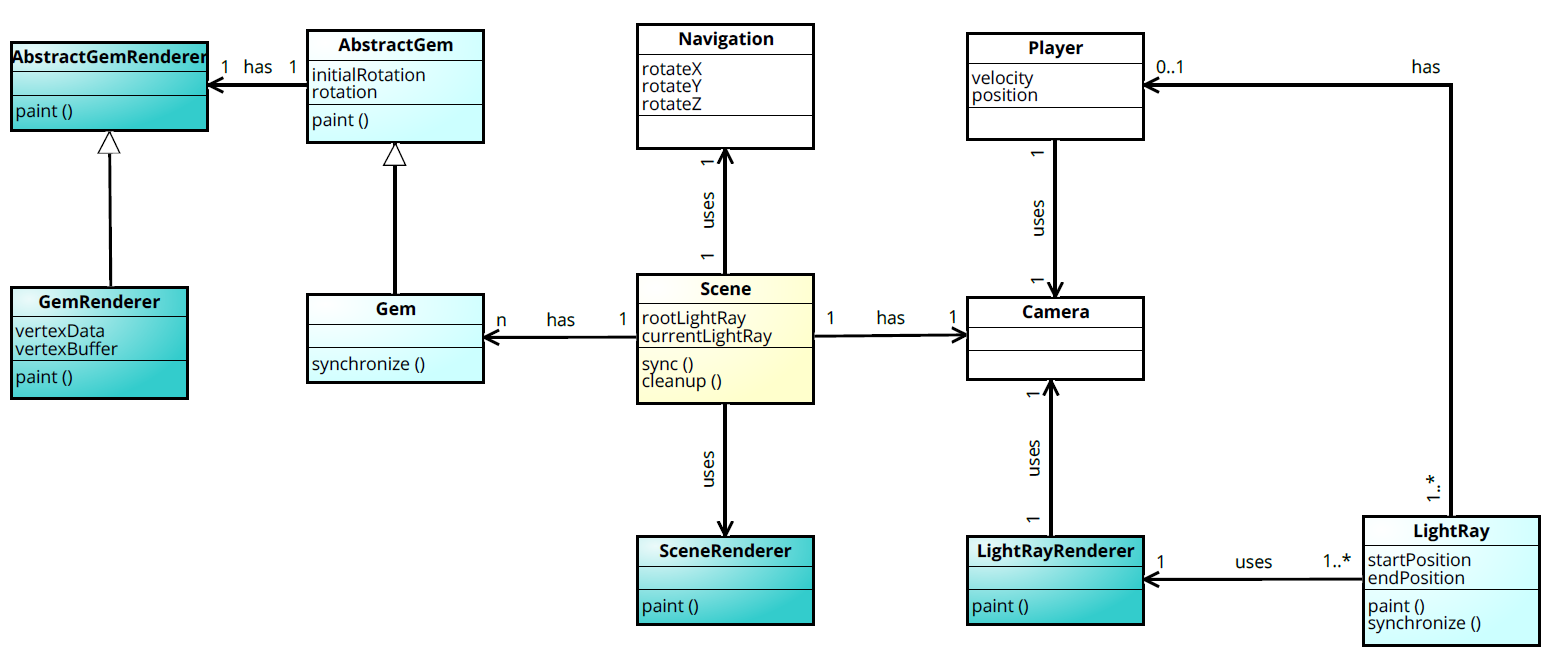
\includegraphics[width=\textwidth, height=0.35\textheight, keepaspectratio]{images/klassendiagramm}
			\caption{Niedrige Framerate}
		\end{subfigure}
		\begin{subfigure}{\textwidth}
			\centering
			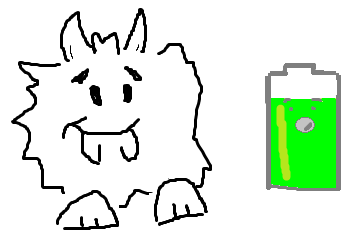
\includegraphics[width=\textwidth, height=0.35\textheight, keepaspectratio]{images/akkufresser}
			\caption{Akkufresse}
		\end{subfigure}
	\end{figure}
}


\begin{frame}{Lösungskonzepte}

\end{frame}

\begin{frame}{Statusupdate zur Entwicklung}

\end{frame}

\begin{frame}{Technische Herausforderungen}

\end{frame}

\begin{frame}{Detaillierter Lösungsansatz}

\end{frame}

%\begin{frame}[allowframebreaks]{Bibliographie}
  \bibliographystyle{apalike}
  \bibliography{../../references}
  \vfill
\end{frame}

\end{document}
